% This LaTeX document needs to be compiled with XeLaTeX.
\documentclass[10pt]{article}
\usepackage[utf8]{inputenc}
\usepackage{graphicx}
\usepackage[export]{adjustbox}
\graphicspath{ {./images/} }
\usepackage{amsmath}
\usepackage{amsfonts}
\usepackage{amssymb}
\usepackage[version=4]{mhchem}
\usepackage{stmaryrd}
\usepackage[fallback]{xeCJK}
\usepackage{polyglossia}
\usepackage{fontspec}
\setCJKmainfont{Noto Serif CJK TC}

\setmainlanguage{polish}
\setmainfont{CMU Serif}

\title{ARKUSZ PRÓBNEJ MATURY Z OPERONEM MATEMATYKA \\
 POZIOM PODSTAWOWY }

\author{}
\date{}


\begin{document}
\maketitle
LISTOPAD 2019

Za rozwiązanie wszystkich zadań można otrzymać łącznie 50 punktów.

\section*{Życzymy powodzenia!}
Wpisuje zdający przed rozpoczęciem pracy\\
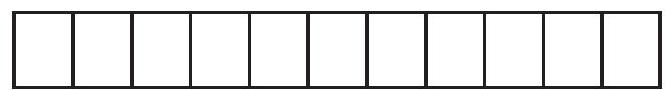
\includegraphics[max width=\textwidth, center]{2024_11_21_e15da647cf0a41077ac3g-01}

PESEL ZDAJĄCEGO\\
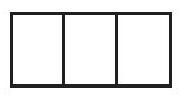
\includegraphics[max width=\textwidth, center]{2024_11_21_e15da647cf0a41077ac3g-01(1)}

KOD\\
ZDAJĄCEGO

\section*{ZADANIA ZAMKNIĘTE}
W zadaniach 1.-25. wybierz i zaznacz jedną poprawną odpowiedź.

\section*{Zadanie 1. (0-1)}
Wartość wyrażenia \((\sqrt{3}-\sqrt{6})^{2}\) jest równa:\\
A. -3\\
B. \(9-6 \sqrt{2}\)\\
C. \(-3-3 \sqrt{2}\)\\
D. 3

\section*{Zadanie 2. (0-1)}
Zbiorem rozwiązań nierówności \(|x| \leq 4\) jest przedział:\\
A. \(\langle-4,4\rangle\)\\
B. \((-\infty, 4)\)\\
C. \((-4,4)\)\\
D. \((-\infty,-4\rangle \cup\langle 4, \infty)\)

\section*{Zadanie 3. (0-1)}
Liczba \(3 \log 2+\log 5^{3}\) jest równa:\\
A. \(\log 7^{3}\)\\
B. \(\log 133\)\\
C. \(3 \log 7\)\\
D. 3

\section*{Zadanie 4. (0-1)}
Cenę pewnego towaru obniżono dwukrotnie: najpierw o \(20 \%\), a następnie o \(10 \%\). Końcowa cena tego towaru jest niższa od ceny początkowej o:\\
A. \(30 \%\)\\
B. \(72 \%\)\\
C. \(28 \%\)\\
D. \(15 \%\)

\section*{Zadanie 5. (0-1)}
Suma liczb \(0,3(7)\) i 0,(7) zapisana w postaci ułamka zwykłego nieskracalnego to:\\
A. \(\frac{52}{45}\)\\
B. \(\frac{115555}{100000}\)\\
C. \(\frac{29}{25}\)\\
D. \(\frac{23}{20}\)

\section*{Zadanie 6. (0-1)}
Funkcja \(f\) przyporządkowuje każdej liczbie naturalnej większej od 1 jej największy dzielnik będący liczbą pierwszą. Który zapis jest fałszywy?\\
A. \(f(22)>f(28)\)\\
B. \(f(21)=f(28)\)\\
C. \(f(25)<10\)\\
D. \(f(28)>9\)

\section*{Zadanie 7. (0-1)}
Osią symetrii wykresu funkcji kwadratowej \(f(x)=\frac{1}{7}(x-5)(x+9)\) jest prosta o równaniu:\\
A. \(x=5\)\\
B. \(x=-9\)\\
C. \(x=-2\)\\
D. \(y=-7\)

\section*{BRUDNOPIS (nie podlega ocenie)}
\begin{center}

\includegraphics[max width=\textwidth]{2024_11_21_e15da647cf0a41077ac3g-03}
\end{center}

\section*{Zadanie 8. (0-1)}
Funkcja liniowa \(f(x)=\left(m^{2}-3\right) x+2\) jest rosnąca wtedy, gdy:\\
A. \(m \in(-\sqrt{3}, \sqrt{3})\)\\
B. \(m \in(-\infty,-\sqrt{3}) \cup(\sqrt{3}, \infty)\)\\
C. \(m \in\{-\sqrt{3}, \sqrt{3}\}\)\\
D. \(m \in(\sqrt{3}, \infty)\)

\section*{Zadanie 9. (0-1)}
W trójkącie równoramiennym \(A B C\), w którym \(|A C|=|B C|\) poprowadzono dwusieczne kątów \(A B C\) i \(A C B\). Dwusieczne te przecięły się w punkcie \(O\) (patrz rysunek).\\
Jeśli \(|\measuredangle B A C|=70^{\circ}\), to miara kąta \(\alpha\) jest równa:\\
A. \(140^{\circ}\)\\
B. \(110^{\circ}\)\\
C. \(55^{\circ}\)\\
D. \(125^{\circ}\)\\
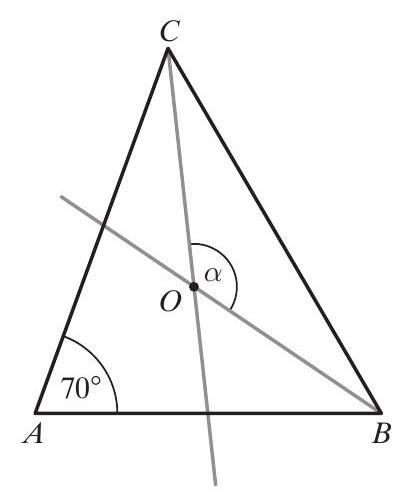
\includegraphics[max width=\textwidth, center]{2024_11_21_e15da647cf0a41077ac3g-04}

\section*{Zadanie 10. (0-1)}
Pole trapezu, jest równe \(20 \mathrm{~cm}^{2}\), a odcinek łączący środki ramion trapezu ma długość 4 cm . Wysokości tego trapezu jest równa:\\
A. 5 cm\\
B. 10 cm\\
C. 2,5 cm\\
D. \(7,5 \mathrm{~cm}\)

\section*{Zadanie 11. (0-1)}
Rozwiązaniem równania \((2 x-5)(3 x+2)=(3 x+2)(x+5)\) są liczby:\\
A. \(-\frac{2}{3}\) i 10\\
B. -5 i 2,5\\
C. \(-5,-\frac{2}{3}\) i 2,5\\
D. -5 i 10

\section*{Zadanie 12. (0-1)}
W trójkącie przedstawionym na rysunku sinus kąta ostrego \(\alpha\) jest równy:\\
A. \(\frac{1}{3}\)\\
B. 3\\
C. \(\sqrt{10}\)\\
D. \(\frac{\sqrt{10}}{10}\)\\
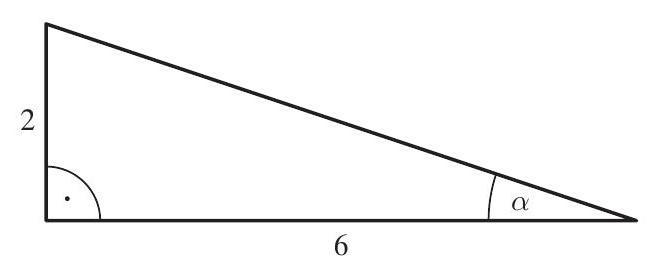
\includegraphics[max width=\textwidth, center]{2024_11_21_e15da647cf0a41077ac3g-04(2)}

\section*{Zadanie 13. (0-1)}
Funkcja, której wykres przedstawiono na rysunku jest rosnąca:\\
A. tylko w przedziale \((-\infty, 0)\)\\
B. tylko w przedziale \((0,+\infty)\)\\
C. w \(R-\{0\}\)\\
D. w każdym z przedziałów \((-\infty, 0) \mathrm{i}(0,+\infty)\)\\
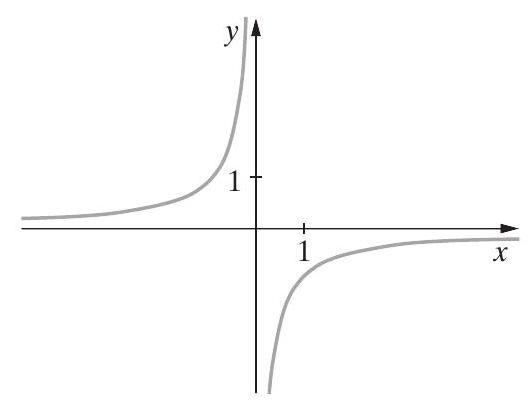
\includegraphics[max width=\textwidth, center]{2024_11_21_e15da647cf0a41077ac3g-04(1)}

\section*{BRUDNOPIS (nie podlega ocenie)}
\begin{center}

\includegraphics[max width=\textwidth]{2024_11_21_e15da647cf0a41077ac3g-05}
\end{center}

\section*{Zadanie 14. (0-1)}
Szósty wyraz ciągu arytmetycznego \(\left(a_{n}\right)\) jest równy zero. Suma jedenastu wyrazów tego ciągu ma wartość:\\
A. 0\\
B. 5\\
C. 11\\
D. -11

\section*{Zadanie 15. (0-1)}
W ciągu geometrycznym, który ma sześć wyrazów, dane są \(a_{3}=\frac{1}{2} \mathrm{i} a_{6}=\frac{1}{16}\). Zatem:\\
A. \(a_{2}=\frac{1}{4}\)\\
B. \(a_{2}=\frac{1}{8}\)\\
C. \(a_{2}=1\)\\
D. \(a_{2}=2\)

\section*{Zadanie 16. (0-1)}
Sześciu robotników wykonało pewną pracę w ciągu 6 godzin i 20 minut. Ośmiu robotników pracujących z taką samą wydajnością wykona tę samą pracę w ciągu:\\
A. 8 godzin i 26 minut\\
B. 4 godzin i 45 minut\\
C. 4 godzin i 20 minut\\
D. 4 godzin i 40 minut

\section*{Zadanie 17. (0-1)}
Stosunek obwodów dwóch sześciokątów foremnych wynosi \(\frac{3}{4}\), a długość boku większego z nich jest równa 12 cm . Mniejszy sześciokąt foremny ma bok długości:\\
A. 27 cm\\
B. 48 cm\\
C. 16 cm\\
D. 9 cm

\section*{Zadanie 18. (0-1)}
Funkcję \(f(x)\) przesunięto wzdłuż osi układu współrzędnych, otrzymując funkcję o wzorze \(g(x)=f(x+4)\). Wobec tego funkcję \(f(x)\) przesunięto o:\\
A. 4 jednostki w prawo\\
B. 4 jednostki w górę\\
C. 4 jednostki w lewo\\
D. 4 jednostki w dół

\section*{Zadanie 19. (0-1)}
Równanie \(\frac{x^{2}-9}{x-3}=0\) :\\
A. nie ma rozwiązań\\
B. ma dokładnie jedno rozwiązanie\\
C. ma dokładnie dwa rozwiązania\\
D. ma dokładnie trzy rozwiązania

\section*{Zadanie 20. (0-1)}
Bok trójkąta równobocznego ma długość 8 cm . Odległość środka ciężkości tego trójkąta od jego boków jest równa:\\
A. \(2 \frac{2}{3} \mathrm{~cm}\)\\
B. \(\frac{4 \sqrt{3}}{3} \mathrm{~cm}\)\\
C. \(\frac{8 \sqrt{3}}{3} \mathrm{~cm}\)\\
D. \(4 \sqrt{3} \mathrm{~cm}\)

\section*{BRUDNOPIS (nie podlega ocenie)}
\begin{center}

\includegraphics[max width=\textwidth]{2024_11_21_e15da647cf0a41077ac3g-07}
\end{center}

\section*{Zadanie 21. (0-1)}
Mediana uporządkowanego zestawu danych: \(4,6, a, b, 8,9\) wynosi 7,5 . Brakującymi wartościami \(a\) i \(b\) mogą być:\\
A. \(a=6, b=6\)\\
B. \(a=6, b=7\)\\
C. \(a=6, b=8\)\\
D. \(a=7, b=8\)

\section*{Zadanie 22. (0-1)}
Przekątna sześcianu ma długość 6 cm . Objętość tego sześcianu jest równa:\\
A. \(24 \sqrt{3} \mathrm{~cm}^{3}\)\\
B. \(24 \mathrm{~cm}^{3}\)\\
C. \(72 \sqrt{3} \mathrm{~cm}^{3}\)\\
D. \(72 \mathrm{~cm}^{3}\)

\section*{Zadanie 23. (0-1)}
Kąt rozwarcia stożka jest równy \(30^{\circ}\), a tworząca tego stożka ma długość 8 cm . Pole przekroju osiowego tego stożka wynosi:\\
A. \(64 \mathrm{~cm}^{2}\)\\
B. \(32 \mathrm{~cm}^{2}\)\\
C. \(16 \mathrm{~cm}^{2}\)\\
D. \(16 \sqrt{3} \mathrm{~cm}^{2}\)

\section*{Zadanie 24. (0-1)}
Trzycyfrowy kod aktywacyjny bramy wejściowej ma następującą postać: litera, cyfra, litera. Litera jest wybierana spośród 24 liter alfabetu i może się w kodzie powtarzać, a cyfra jest dowolna. Ile różnych kodów można w ten sposób utworzyć?\\
A. 58\\
B. 480\\
C. 5760\\
D. 586

\section*{Zadanie 25. (0-1)}
Rzucono 10 razy standardową sześcienną kostką do gry. Średnia arytmetyczna liczb oczek uzyskanych w pierwszych 6 rzutach była równa 3,5, a średnia arytmetyczna liczb oczek uzyskanych w kolejnych 4 rzutach to 4,5 . Srednia arytmetyczna liczb oczek w 10 rzutach wynosi:\\
A. 4,1\\
B. 4,0\\
C. 3,9\\
D. 3,8

\section*{BRUDNOPIS (nie podlega ocenie)}
\begin{center}

\includegraphics[max width=\textwidth]{2024_11_21_e15da647cf0a41077ac3g-09}
\end{center}

\section*{ZADANIA OTWARTE}
Rozwiązania zadań 26.-34. należy zapisać w wyznaczonych miejscach pod treścią zadania.

\section*{Zadanie 26. (0-2)}
Rozwiąż nierówność \(2^{13} \cdot x-3 \cdot 4^{6}<8^{4}(3 x-5)\).

\begin{center}
\begin{tabular}{|c|c|c|c|c|c|c|c|c|c|c|c|c|c|c|c|c|c|c|c|c|c|c|c|c|c|c|c|c|c|}
\hline
 &  &  &  &  &  &  &  &  &  &  &  &  &  &  &  &  &  &  &  &  &  &  &  &  &  &  &  &  &  \\
\hline
 &  &  &  &  &  &  &  &  &  &  &  &  &  &  &  &  &  &  &  &  &  &  &  &  &  &  &  &  &  \\
\hline
 &  &  &  &  &  &  &  &  &  &  &  &  &  &  &  &  &  &  &  &  &  &  &  &  &  &  &  &  &  \\
\hline
 &  &  &  &  &  &  &  &  &  &  &  &  &  &  &  &  &  &  &  &  &  &  &  &  &  &  &  &  &  \\
\hline
 &  &  &  &  &  &  &  &  &  &  &  &  &  &  &  &  &  &  &  &  &  &  &  &  &  &  &  &  &  \\
\hline
 &  &  &  &  &  &  &  &  &  &  &  &  &  &  &  &  &  &  &  &  &  &  &  &  &  &  &  &  &  \\
\hline
 &  &  &  &  &  &  &  &  &  &  &  &  &  &  &  &  &  &  &  &  &  &  &  &  &  &  &  &  &  \\
\hline
 &  &  &  &  &  &  &  &  &  &  &  &  &  &  &  &  &  &  &  &  &  &  &  &  &  &  &  &  &  \\
\hline
 &  &  &  &  &  &  &  &  &  &  &  &  &  &  &  &  &  &  &  &  &  &  &  &  &  &  &  &  &  \\
\hline
 &  &  &  &  &  &  &  &  &  &  &  &  &  &  &  &  &  &  &  &  &  &  &  &  &  &  &  &  &  \\
\hline
 &  &  &  &  &  &  &  &  &  &  &  &  &  &  &  &  &  &  &  &  &  &  &  &  & 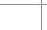
\includegraphics[max width=\textwidth]{2024_11_21_e15da647cf0a41077ac3g-10(2)}
 &  & 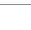
\includegraphics[max width=\textwidth]{2024_11_21_e15da647cf0a41077ac3g-10}
 &  &  \\
\hline
 &  &  &  &  &  &  &  &  &  &  &  &  &  &  &  &  &  &  &  &  &  &  &  &  & 
\includegraphics[max width=\textwidth]{2024_11_21_e15da647cf0a41077ac3g-10(1)}
 &  & 
\includegraphics[max width=\textwidth]{2024_11_21_e15da647cf0a41077ac3g-10(3)}
 &  &  \\
\hline
 &  &  &  &  &  &  &  &  &  &  &  &  &  &  &  &  &  &  &  &  &  &  &  &  & 
\includegraphics[max width=\textwidth]{2024_11_21_e15da647cf0a41077ac3g-10(4)}
 &  &  &  &  \\
\hline
 &  &  &  &  &  &  &  &  &  &  &  &  &  &  &  &  &  &  &  &  &  &  &  &  &  &  &  &  &  \\
\hline
\end{tabular}
\end{center}

Odpowiedź:

\section*{Zadanie 27. (0-2)}
Na trójkącie o bokach długości \(\sqrt{5}, \sqrt{15}, \sqrt{10}\) opisano okrąg. Oblicz długość promienia tego okregu.

\begin{center}
\begin{tabular}{|c|c|c|c|c|c|c|c|c|c|c|c|c|c|c|c|c|c|c|c|c|c|c|c|c|c|c|c|c|c|}
\hline
 &  &  &  &  &  &  &  &  &  &  &  &  &  &  &  &  &  &  &  &  &  &  &  &  &  &  &  &  &  \\
\hline
 &  &  &  &  &  &  &  &  &  &  &  &  &  &  &  &  &  &  &  &  &  &  &  &  &  &  &  &  &  \\
\hline
 &  &  &  &  &  &  &  &  &  &  &  &  &  &  &  &  &  &  &  &  &  &  &  &  &  &  &  &  &  \\
\hline
 &  &  &  &  &  &  &  &  &  &  &  &  &  &  &  &  &  &  &  &  &  &  &  &  &  &  &  &  &  \\
\hline
 &  &  &  &  &  &  &  &  &  &  &  &  &  &  &  &  &  &  &  &  &  &  &  &  &  &  &  &  &  \\
\hline
 &  &  &  &  &  &  &  &  &  &  &  &  &  &  &  &  &  &  &  &  &  &  &  &  &  &  &  &  &  \\
\hline
 &  &  &  &  &  &  &  &  &  &  &  &  &  &  &  &  &  &  &  &  &  &  &  &  &  &  &  &  &  \\
\hline
 &  &  &  &  &  &  &  &  &  &  &  &  &  &  &  &  &  &  &  &  &  &  &  &  &  &  &  &  &  \\
\hline
 &  &  &  &  &  &  &  &  &  &  &  &  &  &  &  &  &  &  &  &  &  &  &  &  &  &  &  &  &  \\
\hline
 &  &  &  &  &  &  &  &  &  &  &  &  &  &  &  &  &  &  &  &  &  &  &  &  &  &  &  &  &  \\
\hline
 &  &  &  &  &  &  &  &  &  &  &  &  &  &  &  &  &  &  &  &  &  &  &  &  &  &  &  &  &  \\
\hline
 &  &  &  &  &  &  &  &  &  &  &  &  &  &  &  &  &  &  &  &  &  &  &  &  &  &  &  &  &  \\
\hline
 &  &  &  &  &  &  &  &  &  &  &  &  &  &  &  &  &  &  &  &  &  &  &  &  &  &  &  &  &  \\
\hline
 &  &  &  &  &  &  &  &  &  &  &  &  &  &  &  &  &  &  &  &  &  &  &  &  &  &  &  &  &  \\
\hline
\end{tabular}
\end{center}

Odpowiedź: \(\qquad\)

\section*{Zadanie 28. (0-2)}
Sprawdź, czy punkty \(A(-2,3), B(2,5), C(2 \sqrt{2}, 4+\sqrt{2})\) są współliniowe.\\

\includegraphics[max width=\textwidth, center]{2024_11_21_e15da647cf0a41077ac3g-11}

Odpowiedź: \(\qquad\)

\section*{Zadanie 29. (0-2)}
Uzasadnij, że równanie \(x^{2}+(a-1) x-a=0\) dla dowolnej liczby rzeczywistej \(a\) ma przynajmniej jedno rozwiązanie.

\begin{center}
\begin{tabular}{|c|c|c|c|c|c|c|c|c|c|c|c|c|c|c|c|c|c|c|c|c|c|c|c|}
\hline
 &  &  &  &  &  &  &  &  &  &  &  &  &  &  &  &  &  &  &  &  &  &  &  \\
\hline
 &  &  &  &  &  &  &  &  &  &  &  &  &  &  &  &  &  &  &  &  &  &  &  \\
\hline
 &  &  &  &  &  &  &  &  &  &  &  &  &  &  &  &  &  &  &  &  &  &  &  \\
\hline
- &  &  &  &  &  &  &  &  &  &  &  &  &  &  &  &  &  &  &  &  &  &  &  \\
\hline
 &  &  &  &  &  &  &  &  &  &  &  &  &  &  &  &  &  &  &  &  &  &  &  \\
\hline
- &  &  &  &  &  &  &  &  &  &  &  &  &  &  &  &  &  &  &  &  &  &  &  \\
\hline
 &  &  &  &  &  &  &  &  &  &  &  &  &  &  &  &  &  &  &  &  &  &  &  \\
\hline
 &  &  &  &  &  &  &  &  &  &  &  &  &  &  &  &  &  &  &  &  &  &  &  \\
\hline
- &  &  &  &  &  &  &  &  &  &  &  &  &  &  &  &  &  &  &  &  &  &  &  \\
\hline
 &  &  &  &  &  &  &  &  &  &  &  &  &  &  &  &  &  &  &  &  &  &  &  \\
\hline
- &  &  &  &  &  &  &  &  &  &  &  &  &  &  &  &  &  &  &  &  &  &  &  \\
\hline
 &  &  &  &  &  &  &  &  &  &  &  &  &  &  &  &  &  &  &  &  &  &  &  \\
\hline
 &  &  &  &  &  &  &  &  &  &  &  &  &  &  &  &  &  &  &  &  &  &  &  \\
\hline
 &  &  &  &  &  &  &  &  &  &  &  &  &  &  &  &  &  &  &  &  &  &  &  \\
\hline
 &  &  &  &  &  &  &  &  &  &  &  &  &  &  &  &  &  &  &  &  &  &  &  \\
\hline
 &  &  &  &  &  &  &  &  &  &  &  &  &  &  &  &  &  &  &  &  &  &  &  \\
\hline
 &  &  &  &  &  &  &  &  &  &  &  &  &  &  &  &  &  &  &  &  &  &  &  \\
\hline
 &  &  &  &  &  &  &  &  &  &  &  &  &  &  &  &  &  &  &  &  &  &  &  \\
\hline
\end{tabular}
\end{center}

\section*{Zadanie 30. (0-2)}
Suma długości boku kwadratu i jego przekątnej jest równa 1. Oblicz długość przekątnej tego kwadratu. Wynik zapisz w postaci \(a+b \sqrt{c}\).\\

\includegraphics[max width=\textwidth, center]{2024_11_21_e15da647cf0a41077ac3g-12}

Odpowiedź:

\section*{Zadanie 31. (0-2)}
Rzucamy dwa razy symetryczną sześcienną kostką do gry. Oblicz prawdopodobieństwo zdarzenia \(A\) polegającego na tym, że liczba oczek w drugim rzucie jest o dwa większa od liczby oczek w pierwszym rzucie.

\begin{center}
\begin{tabular}{|c|c|c|c|c|c|c|c|c|c|c|c|c|c|c|c|c|c|c|c|c|c|c|}
\hline
 &  &  &  &  &  &  &  &  &  &  & - & 到 &  & - & 到 &  &  & - & - & - &  &  \\
\hline
 &  &  &  &  &  &  &  &  &  &  &  &  &  &  &  &  &  &  &  &  &  &  \\
\hline
 &  &  &  &  &  &  &  &  &  &  &  &  &  &  &  &  &  &  &  &  &  &  \\
\hline
 &  &  &  &  &  &  &  &  &  &  &  &  &  &  &  &  &  &  &  &  &  &  \\
\hline
 &  &  &  &  &  &  &  &  &  &  &  &  &  &  &  &  &  &  &  &  &  &  \\
\hline
 &  &  &  &  &  &  &  &  &  &  &  &  &  &  &  &  &  &  &  &  &  &  \\
\hline
 &  &  &  &  &  &  &  &  &  &  &  &  &  &  &  &  &  &  &  &  &  &  \\
\hline
 &  &  &  &  &  &  &  &  &  &  &  &  &  &  &  &  &  &  &  &  &  &  \\
\hline
 &  &  &  &  &  &  &  &  &  &  &  &  &  &  &  &  &  &  &  &  &  &  \\
\hline
 &  &  &  &  &  &  &  &  &  &  &  &  &  &  &  &  &  &  &  &  &  &  \\
\hline
 &  &  &  &  &  &  &  &  &  &  &  &  &  &  &  &  &  &  &  &  &  &  \\
\hline
 &  &  &  &  &  &  &  &  &  &  &  &  &  &  &  &  &  &  &  &  &  &  \\
\hline
 &  &  &  &  &  &  &  &  &  &  &  &  &  &  &  &  &  &  &  &  &  &  \\
\hline
 &  &  &  &  &  &  &  &  &  &  &  &  &  &  &  &  &  &  &  &  &  &  \\
\hline
 &  &  &  &  &  &  &  &  &  &  &  &  &  &  &  &  &  &  &  &  &  &  \\
\hline
 &  &  &  &  &  &  &  &  &  &  &  &  &  &  &  &  &  &  &  &  &  &  \\
\hline
\end{tabular}
\end{center}

Odpowiedź: \(\qquad\)

\section*{Zadanie 32. (0-4)}
Trzy liczby tworzą ciąg arytmetyczny o różnicy \(r=-4\). Jeśli pierwszą i drugą liczbę powiększymy o 3, a trzecią powiększymy o 4 , to otrzymamy trzy kolejne wyrazy ciągu geometrycznego. Oblicz liczby tworzące ciąg arytmetyczny i ciąg geometryczny.

\begin{center}
\begin{tabular}{|c|c|c|c|c|c|c|c|c|c|c|c|c|c|c|c|c|c|c|c|c|c|c|c|c|c|}
\hline
 &  &  &  &  &  &  &  &  &  &  &  &  &  &  &  &  &  &  &  &  &  &  &  &  &  \\
\hline
 &  &  &  &  &  &  &  &  &  &  &  &  &  &  &  &  &  &  &  &  &  &  &  &  &  \\
\hline
 &  &  &  &  &  &  &  &  &  &  &  &  &  &  &  &  &  &  &  &  &  &  &  &  &  \\
\hline
 &  &  &  &  &  &  &  &  &  &  &  &  &  &  &  &  &  &  &  &  &  &  &  &  &  \\
\hline
 &  &  &  &  &  &  &  &  &  &  &  &  &  &  &  &  &  &  &  &  &  &  &  &  &  \\
\hline
 &  &  &  &  &  &  &  &  &  &  &  &  &  &  &  &  &  &  &  &  &  &  &  &  &  \\
\hline
 &  &  &  &  &  &  &  &  &  &  &  &  &  &  &  &  &  &  &  &  &  &  &  &  &  \\
\hline
- &  &  &  &  &  &  &  &  &  &  &  &  &  &  &  &  &  &  &  &  &  &  &  &  &  \\
\hline
- &  &  &  &  &  &  &  &  &  &  &  &  &  &  &  &  &  &  &  &  &  &  &  &  &  \\
\hline
 &  &  &  &  &  &  &  &  &  &  &  &  &  &  &  &  &  &  &  &  &  &  &  &  &  \\
\hline
- &  &  &  &  &  &  &  &  &  &  &  &  &  &  &  &  &  &  &  &  &  &  &  &  &  \\
\hline
 &  &  &  &  &  &  &  &  &  &  &  &  &  &  &  &  &  &  &  &  &  &  &  &  &  \\
\hline
 &  &  &  &  &  &  &  &  &  &  &  &  &  &  &  &  &  &  &  &  &  &  &  &  &  \\
\hline
\end{tabular}
\end{center}

Odpowiedź:

\section*{Zadanie 33. (0-5)}
Podstawą ostrosłupa \(A B C D E\) jest kwadrat, a spodek \(F\) wysokości \(E F\) ostrosłupa jest środkiem krawędzi \(A D\) (patrz rysunek). Ponadto wiadomo, że każda z dwóch dłuższych krawędzi bocznych tego ostrosłupa ma długość \(12 \sqrt{5} \mathrm{~cm}\) i jest nachylona do płaszczyzny podstawy pod kątem \(60^{\circ}\). Oblicz objętość tego ostrosłupa.\\
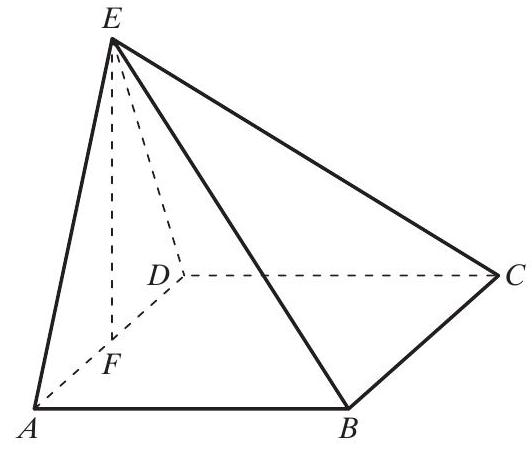
\includegraphics[max width=\textwidth, center]{2024_11_21_e15da647cf0a41077ac3g-13}

\begin{center}
\begin{tabular}{|c|c|c|c|c|c|c|c|c|c|c|c|c|c|c|c|c|c|c|c|c|c|c|c|c|c|c|c|c|}
\hline
 &  &  &  &  &  &  &  &  &  &  &  &  &  &  &  &  &  &  &  &  &  &  &  &  &  &  &  &  \\
\hline
 &  &  &  &  &  &  &  &  &  &  &  &  &  &  &  &  &  &  &  &  &  &  &  &  &  &  &  &  \\
\hline
 &  &  &  &  &  &  &  &  &  &  &  &  &  &  &  &  &  &  &  &  &  &  &  &  &  &  &  &  \\
\hline
 &  &  &  &  &  &  &  &  &  &  &  &  &  &  &  &  &  &  &  &  &  &  &  &  &  &  &  &  \\
\hline
 &  &  &  &  &  &  &  &  &  &  &  &  &  &  &  &  &  &  &  &  &  &  &  &  &  &  &  &  \\
\hline
 &  &  &  &  &  &  &  &  &  &  &  &  &  &  &  &  &  &  &  &  &  &  &  &  &  &  &  &  \\
\hline
 &  &  &  &  &  &  &  &  &  &  &  &  &  &  &  &  &  &  &  &  &  &  &  &  &  &  &  &  \\
\hline
 &  &  &  &  &  &  &  &  &  &  &  &  &  &  &  &  &  &  &  &  &  &  &  &  &  &  &  &  \\
\hline
 &  &  &  &  &  &  &  &  &  &  &  &  &  &  &  &  &  &  &  &  &  &  &  &  &  &  &  &  \\
\hline
- &  &  &  &  &  &  &  &  &  &  &  &  &  &  &  &  &  &  &  &  &  &  &  &  &  &  &  &  \\
\hline
- &  &  &  &  &  &  &  &  &  &  &  &  &  &  &  &  &  &  &  &  &  &  &  &  &  &  &  &  \\
\hline
 &  &  &  &  &  &  &  &  &  &  &  &  &  &  &  &  &  &  &  &  &  &  &  &  &  &  &  &  \\
\hline
 &  &  &  &  &  &  &  &  &  &  &  &  &  &  &  &  &  &  &  &  &  &  &  &  &  &  &  &  \\
\hline
 &  &  &  &  &  &  &  &  &  &  &  &  &  &  &  &  &  &  &  &  &  &  &  &  &  &  &  &  \\
\hline
\end{tabular}
\end{center}

Odpowiedź:

\section*{Zadanie 34. (0-4)}
W gospodarstwie ogrodniczym zapakowano 480 róż do pewnej liczby kartonów. Gdyby jednak do każdego kartonu włożono o 3 róże mniej, to do zapakowania tej samej ilości róż należałoby użyć o 8 kartonów więcej. Do ilu kartonów zapakowano pierwotnie róże i ile róż było w każdym kartonie?\\

\includegraphics[max width=\textwidth, center]{2024_11_21_e15da647cf0a41077ac3g-14}

Odpowiedź: \(\qquad\)

\section*{BRUDNOPIS (nie podlega ocenie)}

\includegraphics[max width=\textwidth, center]{2024_11_21_e15da647cf0a41077ac3g-15}\\
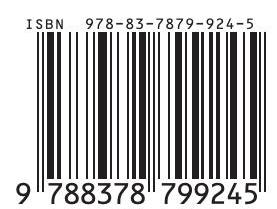
\includegraphics[max width=\textwidth, center]{2024_11_21_e15da647cf0a41077ac3g-16}


\end{document}